\section{Einleitung}
In der Computergrafik werden dreidimensionale Modelle als Polygonen-Netz (Polygonal Mesh) dargestellt, um diese auf einem zweidimensionalen Bildschirm darzustellen. Die Oberfl\"ache eines Modells wird dabei mit Hilfe von Polygonen angen\"ahert. H\"aufig werden daf\"ur Dreiecks-Netze (Triangle Mesh) verwendet, wobei die Fl\"achen mit Dreiecken nachmodelliert werden, siehe Abbildung \ref{fig:dolphintrianglemesh}. 
\\Ein solches Netz besteht aus den Eckpunkten der einzelnen Dreiecke, den Vertices. Diese werden durch Kanten (Edges) verbunden und bilden damit die Polygonalfl\"achen, auch Faces genannt. 

\begin{figure}[h]
	\centering
	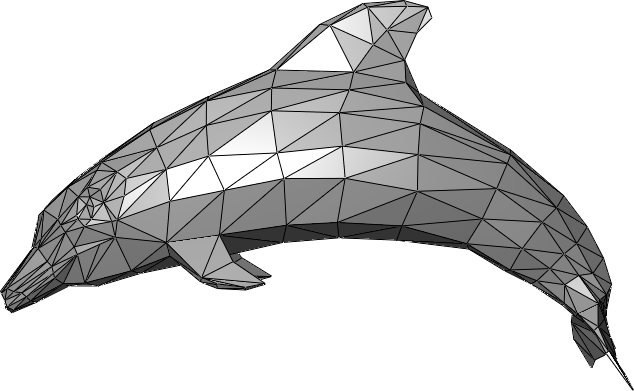
\includegraphics[width=0.7\linewidth]{Images/Dolphin_triangle_mesh}
	\caption[Beispiel eines Polygonen-Netzes]{Beispiel eines Dreiecks-Polygonen-Netz, von \cite{WikipediaDolphin1}}
	\label{fig:dolphintrianglemesh}
\end{figure}

\section{Unity}
Unity ist eine Spiele-Engine mit eingebauter Entwicklungsumgebung f\"ur 2D-, 3D- und VR-Spiele/-Simulationen. Die Engine kommt mit einem eigenen Editor, in welchem diverse Szenarien erstellt und bearbeitet werden k\"onnen. Des Weiteren unterst\"utzt Unity selbst programmierte Scripte auf der Grundlage von C\#.
\subsection{Meshes in Unity}
Unity bietet die M\"oglichkeit, mit Hilfe von selbstgeschriebenen Scripten eigene 3D-Modelle zur Laufzeit erstellen zu lassen. Daf\"ur stellt Unity ein eigenes Mesh-System zur Verf\"ugung, basierend auf Dreiecksnetzen, die \textit{UnityEngine.Mesh}-Klasse. Damit diese ein Mesh rendern kann, erwartet das Mesh ein \textit{UnityEngine.Vector3}-Array f\"ur die Vertices, wobei ein \textit{Vector3} einen Punkt im dreidimensionalen Raum darstellt und ein \textit{int}-Array, das die Reihenfolge der Vertices (\"uber die Indices der Vertices) f\"ur die Dreiecke festlegt.   
\\
Der folgende Code zeigt beispielhaft, wie ein Unity-Mesh erzeugt werden kann:
\begin{lstlisting}
public void CreateMesh()
{
	//--- Der Vollstaendigkeit halber vorhanden
	meshFilter = gameObject.GetComponent<MeshFilter>();
	if (meshFilter == null)
		meshFilter = gameObject.AddComponent<MeshFilter>();

	//--- vom MeshFilter zum Mesh
	mesh = meshFilter.sharedMesh;
	if (mesh == null)
		mesh = new Mesh { name = "Quad" };

	//--- MeshRenderer holen
	meshRenderer = this.gameObject.GetComponent<MeshRenderer>();
	if (meshRenderer == null)
		meshRenderer = gameObject.AddComponent<MeshRenderer>();

	//--- Mesh zusammenstellen
	//--- Vertices/Points
	var P0 = new Vector3(0, 0, 0);
	var P1 = new Vector3(0, 1, 0);
	var P2 = new Vector3(1, 0, 0);
	var P3 = new Vector3(1, 1, 0);
	
	var verticies = new List<Vector3> { P0, P1, P2, P3 };

	//--- Triangles
	var triangles = new List<int>();

	triangles.Add(0);
	triangles.Add(1);
	triangles.Add(2);
	triangles.Add(2);
	triangles.Add(1);
	triangles.Add(3);

	//--- Mesh befuellen
	mesh.Clear();
	//--- Vertices zuweisen
	mesh.vertices = verticies.ToArray();
	//--- Triangles zuweisen
	mesh.triangles = triangles.ToArray();
	//--- Mesh dem MeshFilter zuweisen
	meshFilter.sharedMesh = mesh;
}
\end{lstlisting}

Und liefert folgendes Ergebnis:
\begin{figure}[h]
	\centering
	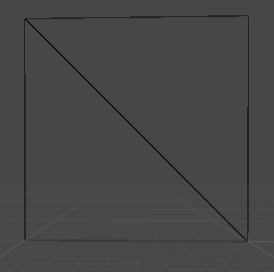
\includegraphics[width=0.35\linewidth]{Images/UnityQuadWireframe}
	\caption[Die Wireframeansicht des erstellten Meshes]{Die Wireframeansicht des erstellten Meshes im Unity Editor}
	\label{fig:unityquadwireframe}
\end{figure}

\subsection{Nachteile von Unity-Meshes}
Die Vorteile bei dieser Herangehensweise sind, dass die von Unity verwendeten Netze auch bei gr\"o{\ss}eren Netzen vergleichsweise wenig Speicherplatz ben\"otigen, da dieser Ansatz auf eine direkte Repr\"asentation von Faces und Edges verzichtet. Daraus ergeben sich einige Nachteile. Durch die fehlende Referenz auf die Polygonenfl\"achen sind Operationen auf Face-Ebene, wie eine Nachbarsuche, Abfragen auf alle Punkte Kanten oder die Unterteilung einzelner Polygonen in kleinere Einheiten (auch ,,Subdivision'' genannt), sehr Zeitintensiv, weshalb sich solche F\"alle nicht f\"ur Echtzeitanwendungen eignen. Des Weiteren stehen die Vertices im Unity-Mesh in keinem topographischen Zusammenhang, wodurch eine Iteration \"uber das gesamte Netz erschwert wird, um beispielsweise zusammenh\"angende Punkte zu bearbeiten.
